\documentclass{article}
\usepackage{graphicx} % Required for inserting images
\usepackage{amsmath}
\usepackage[margin=1in]{geometry}
\usepackage{listings}
\usepackage{array}
\usepackage{glossaries}

\makeatletter
\renewenvironment{thebibliography}[1]
{% \section*{\refname}% <-- This line adds the section heading, remove it
  \list{\@biblabel{\@arabic\c@enumiv}}%
       {\settowidth\labelwidth{\@biblabel{#1}}%
        \leftmargin\labelwidth
        \advance\leftmargin\labelsep
        \@openbib@code
        \usecounter{enumiv}%
        \let\p@enumiv\@empty
        \renewcommand\theenumiv{\@arabic\c@enumiv}}%
  \sloppy
  \clubpenalty4000
  \@clubpenalty \clubpenalty
  \widowpenalty4000%
  \sfcode`\.\@m}
{\def\@noitemerr
  {\@latex@warning{Empty `thebibliography' environment}}%
 \endlist}
\makeatother


% \usepackage{glossaries-extra}  % Uncomment if you need extra features
\makeglossaries  % Initialize the glossary system
\newglossaryentry{productDef}{
  name={Product Definition},
  description={Overview of the full product concept.}
}
\newglossaryentry{summary}{
  name={Product Summary},
  description={Summary of problem}
}
\newglossaryentry{identification}{
  name={Identification},
  description={Identification of the product}
}
\newglossaryentry{users}{
  name={Users},
  description={Definition of who will benefit from product}
}
\newglossaryentry{interfaces}{
  name={Interfaces},
  description={How the user will interact with the product}
}
\newglossaryentry{userreq}{
  name={User Requirements},
  description={What the user needs to know}
}
\newglossaryentry{customerneeds}{
  name={Customer Needs},
  description={What the user needs out of the product}
}
\newglossaryentry{projectdefinition}{
  name={Project Definition},
  description={Overview of the project}
}
\newglossaryentry{projectsummary}{
  name={Summary},
  description={Summary of what will be explored in the project}
}
\newglossaryentry{limitations}{
  name={Constraints and Limitations},
  description={Constraints and limitations of the project's execution}
}
\newglossaryentry{assumptions}{
  name={Assumptions and Dependencies},
  description={Assumptions and dependencies within the project}
}
\newglossaryentry{arch}{
  name={Architecture},
  description={Architecture of the project}
}
\newglossaryentry{design}{
  name={Design Justification},
  description={Justification of design choices}
}
\newglossaryentry{specs}{
  name={Specifications},
  description={Specifications of the project}
}
\newglossaryentry{schedule}{
  name={Project Schedule},
  description={Gantt chart of timeline}
}
\newglossaryentry{bom}{
  name={Bill of Materials},
  description={Prototype cost}
}
\newglossaryentry{references}{
  name={References},
  description={Sources of the documents reviewed}
}
\newglossaryentry{appendix}{
  name={Appendix},
  description={Extra items}
}
%Document
\begin{document}
\pagestyle{empty}

\vspace*{\fill}   % Centers the title vertically on the page

\begin{center}
    {\LARGE Engineering Requirements Document \\}   % Title in Large font
    \vspace{1cm}         % Space between title and author name
    {\large Lucas Butler \\}  % Author name in a smaller font than the title
    \vspace{1cm}         % Space between author name and date
    {\large \today}      % Today's date in a smaller font
\end{center}

\vspace*{\fill}   % Fill the rest of the page


\newpage

\setcounter{page}{1}
\pagestyle{plain}

\printglossaries
\newpage

\section{\gls{productDef}}
\subsection{\gls{summary}}
\quad In the United States, cardiac disease produces a significant number of casualties, nearly 700,000 deaths a year \cite{cdc}. Currently, anomalies such as irregular heart rhythms (arrhythmia) and blood flow blockages (myocardial infarction) are monitored through the collection and classification of Electrocardiogram signals \cite{typesofcardiac}. These signals are typically collected in a clinical setting, through electrodes and wires, under the supervision of doctors and nurses, and take a significant amount of time to be sifted through and classified. The current methods require significant effort from medical professionals, yet yields low volumes of treated patients relative to the demand. 
\subsection{\gls{identification}}
In order to alleviate the bottlenecks created by the current system, significant infrastructural improvements must be achieved. To make access of ECG signal acquisition more ubiquitous, Internet of Things (IoT), Cloud, and Machine learning technologies will need to extend upon tradition Digital Signal Processing algorithms and cutting edge computer hardware.

At the edge, a power-efficient ECG sensor node capable of long range data communication can be utilized to collect ECG data. The use of wireless communication will erase the need to enter a clinical setting and make the classification technology available to more patients. It will also eliminate the need for wires and stand-alone monitoring systems, which will reduce tripping hazards in operation settings and reduce asset maintenance costs. 

With wireless data collection and communication, employing a cloud-based approach to monitoring signals will now be feasible. This approach will utilize communication across the web, transmitting data to a centralized database. Data stored would be accessible through a web interface, releasing constraints over location  and providing a comprehensive over view for all patients in a one-stop shop. An optimal approach to development would be in the form of a deployable cloud container that scales with the number of requests for service. This cloud container could be deployed within the hospital or clinical network for internal usage or by a business on a local server for servicing individual patient requests, outside of a clinical setting.

To assist in the prioritization and classification of cases, Machine Learning technologies, such as Convolutional Neural Networks, can operate on the data stored in the cloud server. These neural networks can identify target patterns in signals and predict anomalies with high accuracy. This technology would enable medical professionals to prioritize cases, enabling a greater impact on the front line of cardiovascular disease.

Developing a robust, IoT heart-health monitoring system would increase the quality of life of medical professionals and subjects to cardiovascular disease by improving the efficiency of triage within the health care system, in addition 
to making cardiac telemetry more accessible. 

\newpage
\subsection{\gls{users}}
A versatile ECG signal classification system will serve a wide variety of people including: health professionals, patients at-risk, and the general population.

This technology will be heavily utilized by hospitals and clinics. Centralized monitoring will enable a more informed view for medical professionals to use while making decisions on resource allocation. Automating the collection and detection of anomalies will improve prioritization of patients and provide more opportunity to prevent failure, significantly contributing to the health care effort. Doctors will benefit from additional medical data when discovering root causes and fine-tuning their assessment policies. Introducing this streamlined approach will empower medical professionals to excel in their responsibilities.

Patients will greatly benefit from ubiquitous ECG classification. Those at-risk are typically worried about abnormalities and feel tied to hospitals or clinics for consistent updates. Unrestricted cardiovascular monitoring will relieve this stress by facilitating patient autonomy and fostering a deeper engagement with more enjoyable daily tasks. With improved insight, those at-risk will be able to self-assess the challenges they face during various activities, providing a drastic improvement in the average quality of life. 

Everyone, including those who are not considered at-risk or health professionals, will benefit. Providing deeper insights into cardiovascular health will allow individuals to make better decisions about their eating, exercising and sleeping habits. Athletes and fitness enthusiasts will utilize this information to prep for important matches and improve training regiments. Post-op surgery patients will benefit from smoother recovery, and the Elderly will rest, assured that they are in good health.

\subsection{\gls{interfaces}}
This system extends multiple domains in order to operate effectively. The user interact with a physical sensor, as well as an interface to their Personal Health Information (PHI) using a web-application. Medical professionals will utilize a fully featured dashboard for managing their patients.

Sensor Node: Wireless sensor nodes will be easily operable by patients and practitioners. The connectivity protocol will be simple; turn on the sensor and press a button to initiate the connection, then connect the device through an online portal. An LED indicator on the sensor will indicate the state of connection, communication, and indicate if the battery is getting low.

User Profile: Each patient will have a unique profile. The profiles will employ multi-factor authentication through text message, phone call, or email verification to increase the security of sensitive medical data. Through this unique profile, patients will be able to connect their with medical providers, allowing medical professionals to read and analyze their data. This feature will be enabled at the discretion of the user and can be revoked without external consent, giving users full control over their data. 

Data Presentation: A dashboard for the centralized database will provide a comprehensive overview of heart-health. Medical professionals will have the option to view multiple patients data in realtime, giving them greater control over their awareness. Alerts will notify the professionals about anomalies to enable quick responses. 

\newcolumntype{M}[1]{>{\centering\arraybackslash}p{#1}}

\newpage
\subsection{\gls{userreq}}
\begin{table}[h]
    \centering
    \begin{tabular}{|M{0.3cm}|p{4cm}|p{5cm}|}
        \hline
        \# & Requirement & Description \\
        \hline
        1 & Email & Access to an email account will be necessary for generating a user profile. \\
        \hline
        2 & Phone Number (optional) & Phone numbers will aid in notifying the users of events, authentication when logging in and other security reasons. \\
        \hline
        3 & Internet Access & Access to web for transmitting and receiving health information will be required. \\
        \hline
        4 & Electrical Outlet & Access to power is required for charging the sensor node or host workstation. \\
        \hline
        5 & Computer/Mobile Device with Browser & All services are accessed through a web portal. A device with a web browser is essential. \\ 
        \hline
        6 & Basic Knowledge about Heart Health & A basic understanding of heart-beat and the cardiovascular system is important to get value out of the product. \\
        \hline
        7 & Sensor Node & A wearable capable of collecting ECG signals and transmitting them wirelessly. \\
        \hline
        8 & Hosting & If hosting, use of cloud hosting platforms like AWS or use of personal servers is required for the application to run.\\
        \hline
        9 & Receiver & A local Zigbee receiver than connects to the internet is required to send and receive sensor transmissions.\\
        \hline
    \end{tabular}
    \caption{User Requirements}
    \label{tab:example}
\end{table}

\newpage

\subsection{\gls{customerneeds}}

\begin{table}[h]
    \centering
    \begin{tabular}{|M{0.3cm}|p{4cm}|p{5cm}|}
        \hline
        \# & Requirement & Description \\
        \hline
        1 &  Secure Data Transmission & All data transmission should be encrypted to ensure privacy of user health information. \\
        \hline
        2 & Accurate Classification & Captured signals should be high quality. Classifications of signals should be highly accurate, ensuring customer confidence in the product.  \\
        \hline
        3 & Real Time Updates & Overall system latency should be very low, providing real-time updates on the current state of health. \\
        \hline
        4 & Notifications & A robust notification system that updates both patients and medical professionals when an emergency is occurring.\\
        \hline
        5 & Help Desk Service & A 24/7 assistance service that helps users with setting up the system, troubleshooting issues, and providing additional information to enable thorough extraction of product value. \\ 
        \hline
        6 &  Cloud Storage & Centralized, secure storage of user data to enable ease of access from any device, at any time. \\
        \hline
        7 & Simple, Intuitive UI/UX & The User Experience should reduce as much complexity as possible, giving users easy access to the features they need, while hiding the unhelpful information. \\
        \hline
        8 & Long Battery Life & The system architecture should enable extended range and battery life in at the edge. \\
        \hline
        9 & Data Security & The PHI storage system should have redundancy and robust security protocols to maximize protection of privacy.\\
        \hline
    \end{tabular}
    \caption{Customer Requirements}
\end{table}

\newpage
\section{\gls{projectdefinition}}
\subsection{\gls{projectsummary}}
The focus of implementation will be on the design of the server-side signal processing pipeline. This project will focus on high performance computing implementations of the Zigbee packet parser, signal processing algorithm, and the peak detection algorithm.
\subsection{\gls{limitations}}
There are numerous constraints placed upon this project. Time constraints are a major limitation as researching, designing and developing this project in one semester will allow little room for revision. Technical complexity when implementing the various algorithms will demand extensive troubleshooting and testing. Technical knowledge on each of the subjects explored in the project will limit the effectiveness of the implementation and the performance improvements that are possible. 

Abiding to all the regulations specified by the FDA and HIPAA will also be a challenge due to the shear quantity and limited time to get familiar; this project will focus on the decryption of AES-256, but leave the data storage regulations for later. Due to the lack of developed infrastructure, emulation techniques must be utilized for testing, including creation of artificial signals and network packets. The compute power of the work station used in the project (my laptop) will provide limitations to how fast the processing can be executed. 
\subsection{\gls{assumptions}}
Signal characteristics of ECG are as follows: 0.05-100 Hz, input voltage of 0.5-5.0 mV from the electrode. Various forms of noise such as electrode contact (0-20 Hz), various bodily signals (0.13-3 Hz), and motion artifacts (0-20 Hz) will be present in the signal \cite{ecgfiltering}. Power line noise in the range of 50-60 Hz can be neglected due to battery operation. Using the Nyquist theorem as a baseline, the signal will be sampled at 500 Hz to put us far above 200 Hz, produced by the equation $S = 2 * f$. The data type used to store samples will be a 16-bit integer. HIPAA imposes strict regulations on Personal Health Information and suggests using 256-bit AES as the standard encryption protocol \cite{sprinto}. The network packets that are received will be in the Zigbee format. In regards to heart rate peak detection, the Pan Tompkins algorithm is the most widely used algorithm \cite{pantompkins} and will be used in this implementation.

\newpage
\subsection{\gls{arch}}

\begin{figure}[h]
    \centering
    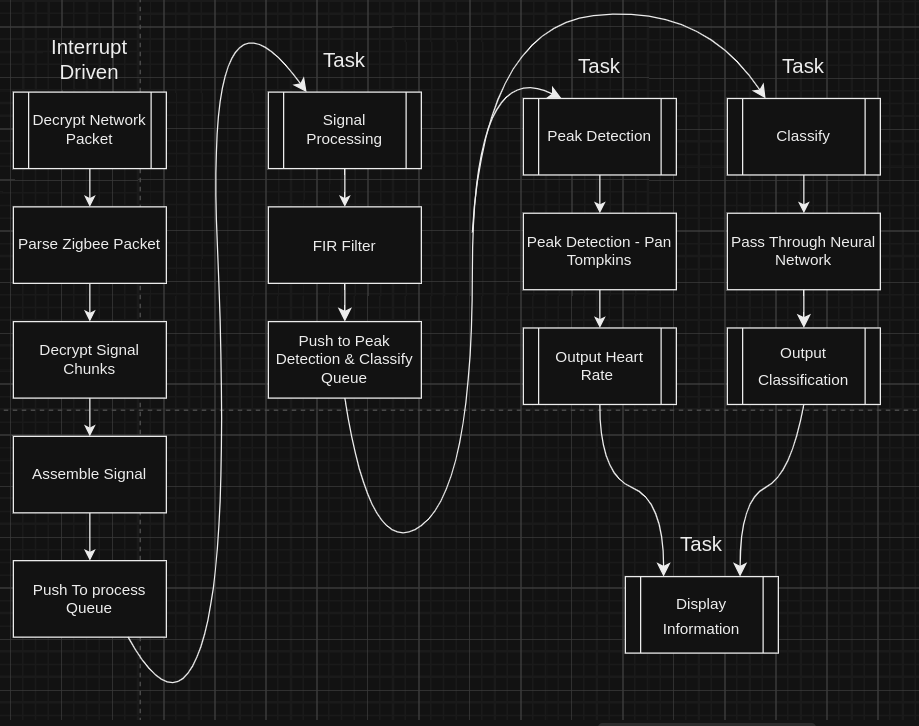
\includegraphics[width=5in, height=4in]{flow1.png}
    \caption{Top level flow of software.}
\end{figure}


\newpage
\subsection{\gls{design}}
Wireless communication protocol selection is a critical design choice for this project. There are various design requirements to consider when choosing a protocol. First, the receiving station must be able to receive signals from multiple sensors simultaneously. Second, the communication protocol must be low-power to maximize the battery life of the sensor. Third, the data rate needs to support transmitting a minimum of 500 samples of 2-byte data per second from the signal acquisition system, yielding a minimum rate of 8 Kbps. 

Wi-Fi and Bluetooth communication protocols were identified as alternatives to Zigbee, but were later found to have issues satisfying the requirements. Wi-Fi is overpowered for data transmission, as normal rates for 802.11b are in the 10s of Mbps range \cite{cisco}, whereas we only require the range of 10s of Kbps transmission per node. Wi-Fi would not be fully utilized, causing power consumption issues in the sensor. Bluetooth Low Energy (BLE) data rates are much closer to our required rate, in the range of 125 Kbps - 2 Mbps \cite{nordic}, and are designed for lower energy consumption. The third option is Zigbee, which has a data rate in the 250 kbps range \cite{ehub}. The main difference between BLE and Zigbee is the network topology. BLE adopts a Master-Slave topology and limits the master to 8 devices for communication \cite{ehub}. This topology allows for many devices to join a system, however, it produces significant bottlenecks due to the lack of freedom that network packets have when traveling through other nodes to reach a destination. On the contrary, Zigbee uses a mesh network topology, which allows data to hop between devices to reach its destination. This topology would decrease latency compared to BLE transmission, keeping users happy. For designing scalable sensor node systems, Zigbee is the best choice.

Signal processing can be carried out in various ways, each with considerations of power efficiency, signal integrity, complexity, and flexibility. One approach that was heavily considered was utilizing hardware and analog filters to remove unwanted artifacts. Analog filters are very efficient in reducing the propagation delay of the signal, however, hardware implementations are generally less iterable due to supply chain delays and the time required for implementation of the circuit. Due to the short project execution time, an implementation that promotes iterability is being prioritized. Another option is sensor-side digital signal processing using a microconverter. Hartmann \cite{analogfilter} demonstrates an implementation where digital filtering was executed using an ADuC842 MicroConverter. Although this implementation provides an effective solution to the signal processing requirements, it consumes energy from the sensor's battery, decreasing the operation time. Switching to a server-side processing pipeline would make two improvements. First, it would yield a minimum power consumption decrease of 3.4\% over Hartmann's design, assuming only the ADuC842 DSP unit is removed. More importantly, utilizing a multi-core processor like the Intel i9 which operates at 5.0 GHz \cite{msi}, instead of a single-cycle chip in the range of 32 kHz, like the ADuC842 \cite{ADUC842}, would enable a significant time reduction in overall system latency. In addition, access to server-side GPUs would enable even lower latency through parallel computation. In conclusion, using server-side signal processing would decrease system latency and increase the operation time of the sensor.

There are various algorithms and filtering techniques capable of signal filtration, each with specific applications. Pradhan et al. \cite{timefreqmethods} conduct an extensive study on which algorithms are best for different ECG classification tasks, finding that the Discrete Wavelet Transform is the most widely used algorithm for general applications, EMD filters are best for more nuanced applications, and that 2-D methods such as the spectrogram, scalogram, and frequency plots are best for deep learning classification tasks. Xiang An and George K. Stylios \cite{filtercomparison} do a more in-depth review of the performance of various algorithms on normal and abnormal ECG signals and find that the Finite Impulse Response (FIR) filter and a self-developed Adaptive filter yield much greater results than the Discrete Wavelet Transform and EMD filter in terms of Signal-to-Noise Ratio improvement, suggesting that either of these options is a better route. Due to the technical complexity of the self-developed Adaptive Filter proposed by An and Stylios, and the more widespread knowledge available in regards to the FIR filter implementation, the FIR filter was chosen for this project.
\par
\newpage
\subsection{\gls{specs}}
\begin{table}[h]
    \centering
    \begin{tabular}{|M{0.3cm}|p{4cm}|p{5cm}|}
        \hline
        \# & Requirement & Ideal Value \\
        \hline
        1 & Target Frequency Band & 0.5-100Hz \\
        \hline
        2 &  Input Signal Voltage & 0.5-5.0 mV \\ 
        \hline
        3 &  Signal Sampling Rate & 500 Hz \\
        \hline
        4 &  Data Encryption & AES-256  \\
        \hline
        5 &  Wireless Connectivity & Zigbee PRO\\
        \hline
        6 &  Wireless Data Transmission of 1 sensor & 8 Kbps \\
        \hline
        7 &  Signal Capture Window & 3 seconds of signal capture for one data batch. \\ 
        \hline
        8 &  Software Optimization & Parallel processing and GPU-accelerated algorithms \\
        \hline
        9 &  FIR Implementation & Nvidia CUDA platform for parallel computing. \\
        \hline
        10 & CPU Specifications & Multi-core (e.g., 16+ cores), High Clock Speed (e.g., 3+ GHz). \\
        \hline
        11 & Data Compression & Lossless compression algorithms for storage optimization. \\
        \hline
        12 & Storage Type & NVMe SSD for primary storage. \\
        \hline
        13 & Data Backup & Regular automated backup system. \\
        \hline
        14 & Signal Integrity & Automated artifact detection system. \\
        \hline
        15 & Storage Capacity & 1TB or higher \\
        \hline
    \end{tabular}
    \caption{Customer Requirements}
\end{table}

\newpage
\subsection{\gls{schedule}}
\begin{figure}[h]
    \centering
    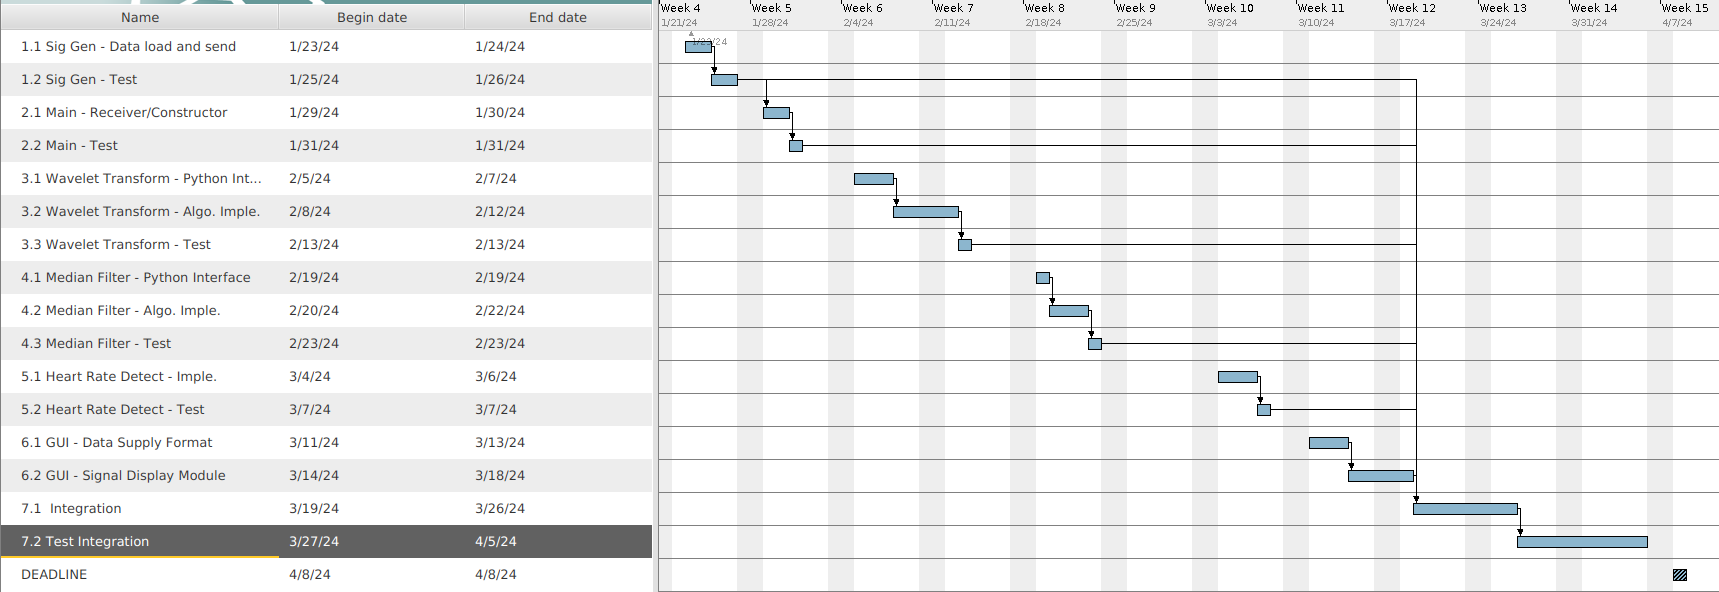
\includegraphics[width=6.5in, height=2.25in]{Gantt.png}
    \caption{Gantt chart of the project.}
\end{figure}
\subsection{\gls{bom}}

\begin{figure}[h]
    \centering
    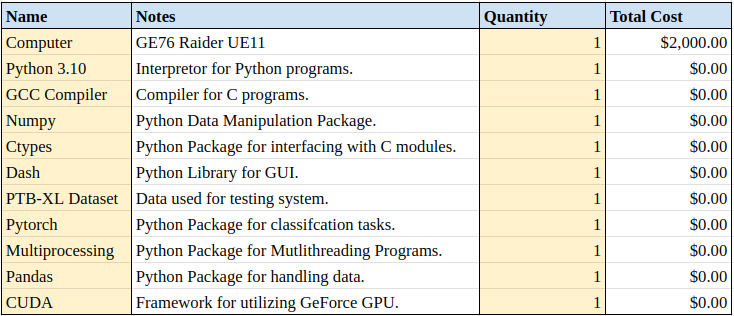
\includegraphics[width=5in, height=2.1in]{BOM.png}
    \caption{Bill of materials for project.}
\end{figure}

\newpage

\section{\gls{references}}
\begin{thebibliography}{13}
        
    \bibitem{cdc}
    Centers for Disease Control and Prevention, "Heart Disease Facts." [Online]. Available: https://www.cdc.gov/heartdisease/facts.htm. [Accessed: Nov. 26, 2023].

    \bibitem{typesofcardiac}
    "Congenital Heart Disease," NHS. [Online]. Available: https://www.nhs.uk/conditions/congenital-heart-disease/. [Accessed: Nov. 26, 2023].

    \bibitem{analogfilter}
    "ECG Front-End Design is Simplified with MicroConverter," Analog Dialogue. [Online]. Available: https://www.analog.com/en/analog-dialogue/articles/ecg-front-end-design-simplified. [Accessed: Nov. 26, 2023].
    
    \bibitem{msi}
    "GE76 Raider (Intel 11th Gen)(GeForce RTX 30 Series)," MSI. [Online]. Available: https://us.msi.com/Laptop/GE76-Raider-11UX. [Accessed: Nov. 26, 2023].

    \bibitem{ADUC842}
    "ADUC842 Datasheet (PDF) - Analog Devices," Electronic Components Datasheet Search. [Online]. Available: https://www.alldatasheet.com/datasheet-pdf/pdf/98398/AD/ADUC842.html. [Accessed: Nov. 26, 2023].
    
    \bibitem{cisco}
    "RF Design Considerations," Cisco Systems, Inc. [Online]. Available: https://www.cisco.com/en/US/docs/solutions/Enterprise/Mobility/emob30dg/RFDesign.html. [Accessed: Nov. 20, 2023].
    
    \bibitem{nordic}
    "The complete guide to Bluetooth Low Energy," Nordic Semiconductor. [Online]. Available: https://response.nordicsemi.com/the-complete-guide-to-bluetooth-low-energy. [Accessed: Nov. 20, 2023].
    
    \bibitem{ehub}
    "Zigbee Vs Bluetooth," ElectronicsHub. [Online]. Available: https://www.electronicshub.org/zigbee-vs-bluetooth/. [Accessed: Nov. 20, 2023].

    \bibitem{sprinto}
    Sprinto, "List of HIPAA Encryption Requirements," Sprinto. [Online]. Available: https://www.sprinto.com/compliance/hipaa-encryption-requirements/. [Accessed: Nov. 26, 2023].

    \bibitem{ecgfiltering}
    S. Nayak, M. K. Soni, and D. Bansal, "Filtering Techniques for ECG Signal Processing," in International Journal of Research in Engineering \& Applied Sciences, vol. 2, no. 2, pp. 671, Feb. 2012. [Online]. Available: http://www.euroasiapub.org. [Accessed: Nov. 20, 2023].
    
    \bibitem{yang}
    Y. -H. Yang, S. -J. Ruan, P. -C. Chen, Y. -T. Liu, and Y. -H. Hsueh, "A Low-Cost Wireless Multichannel Surface EMG Acquisition System," in IEEE Consumer Electronics Magazine, vol. 9, no. 5, pp. 14-19, 1 Sept. 2020, doi: 10.1109/MCE.2020.2986792. [Accessed: Nov. 26, 2023].
    
    \bibitem{timefreqmethods}
    A. Liu, B. K. Pradhan, B. C. Neelappu, J. Sivaraman, D. Kim, and K. Pal, "A Review on the Applications of Time-Frequency Methods in ECG Analysis," in Journal of Healthcare Engineering, vol. 2023, pp. 3145483, Feb. 2023. [Online]. Available: https://doi.org/10.1155/2023/3145483. [Accessed: Nov. 26, 2023].

    \bibitem{filtercomparison}
    An X, K Stylios G., "Comparison of Motion Artefact Reduction Methods and the Implementation of Adaptive Motion Artefact Reduction in Wearable Electrocardiogram Monitoring." Sensors (Basel). 2020 Mar 7;20(5):1468. doi: 10.3390/s20051468. PMID: 32155984; PMCID: PMC7085712. [Accessed: Nov. 26, 2023].

    \bibitem{pantompkins}
    Khan N, Imtiaz MN. "Pan-Tompkins++: A Robust Approach to Detect R-peaks in ECG Signals." arXiv preprint arXiv:2211.03171. 2022. Available at: https://arxiv.org/abs/2211.03171. [Accessed: Nov. 26, 2023].
    
\end{thebibliography}  

\newpage

\section{\gls{appendix}}
\begin{figure}[h]
  \centering
  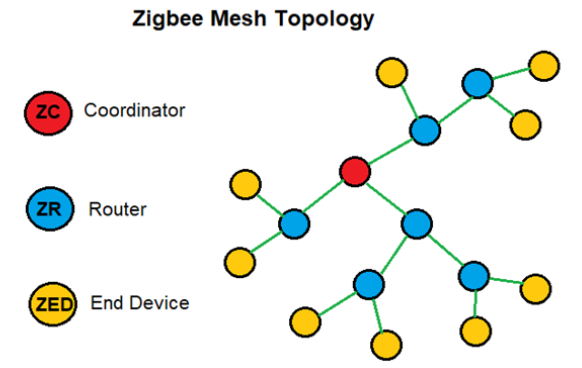
\includegraphics[width=3in, height=2in]{zigbee-topology.png}
\end{figure}

\begin{figure}[h]
  \centering
  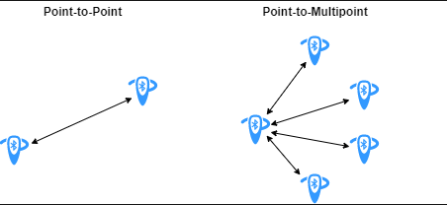
\includegraphics[width=3.5in, height=2in]{bluetooth-topology.png}
\end{figure}

\begin{figure}[h]
  \centering
  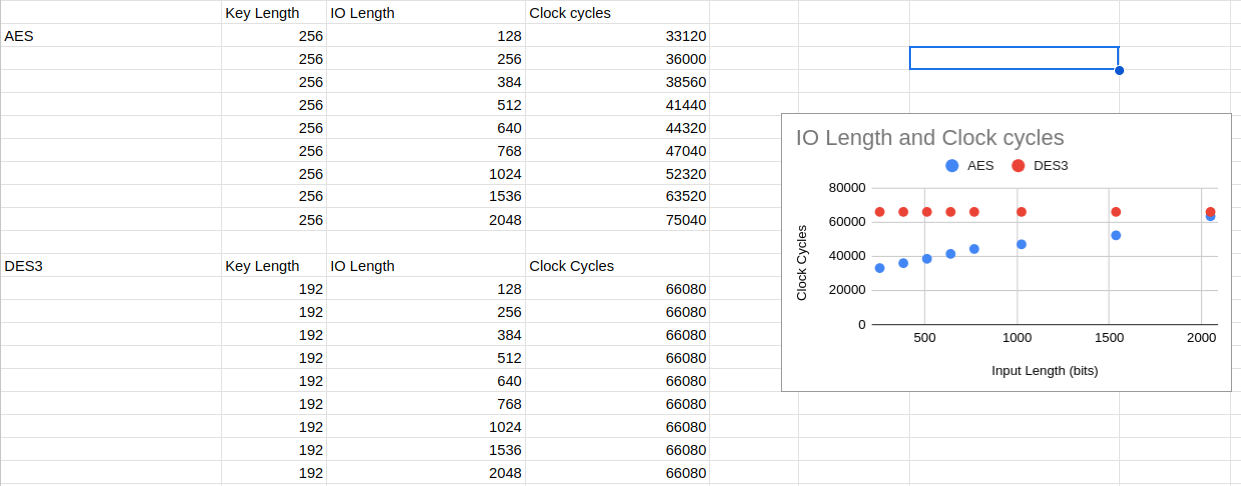
\includegraphics[width=4in, height=2in]{encryption.png}
\end{figure}

\begin{figure}[h]
  \centering
  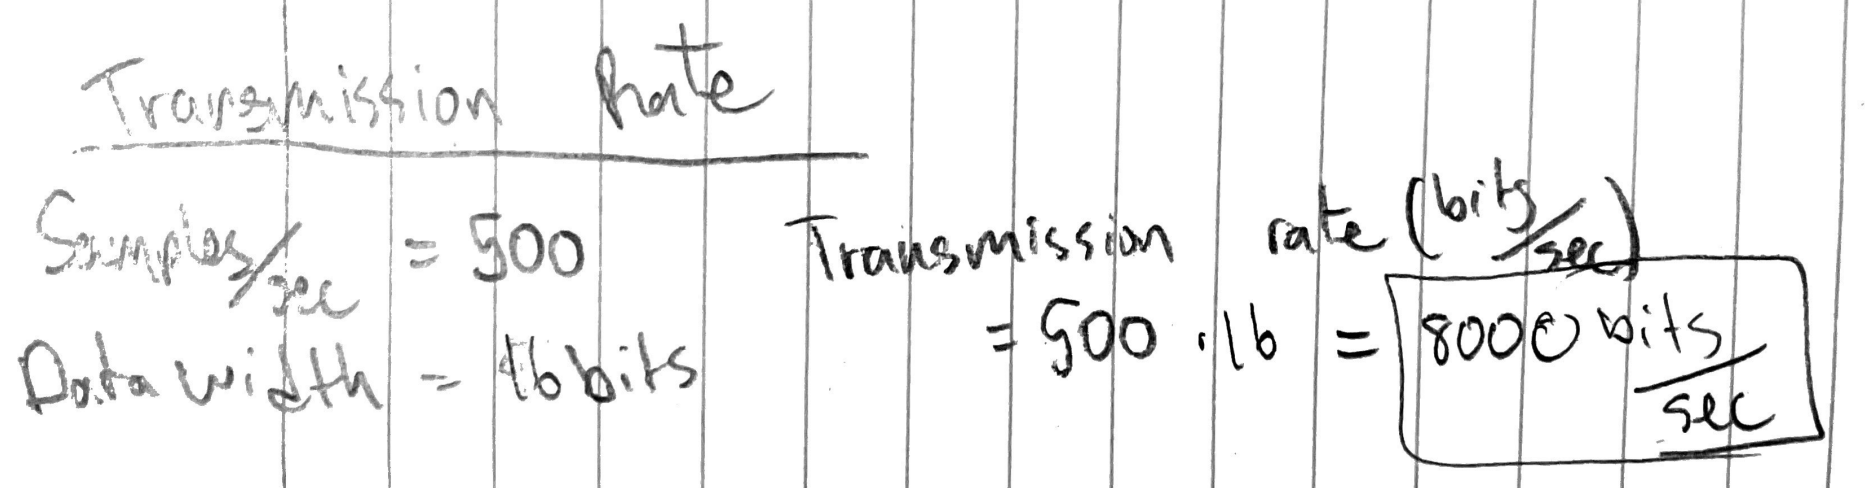
\includegraphics[width=3in, height=1in]{transmission.png}
\end{figure}

\begin{figure}[h]
  \centering
  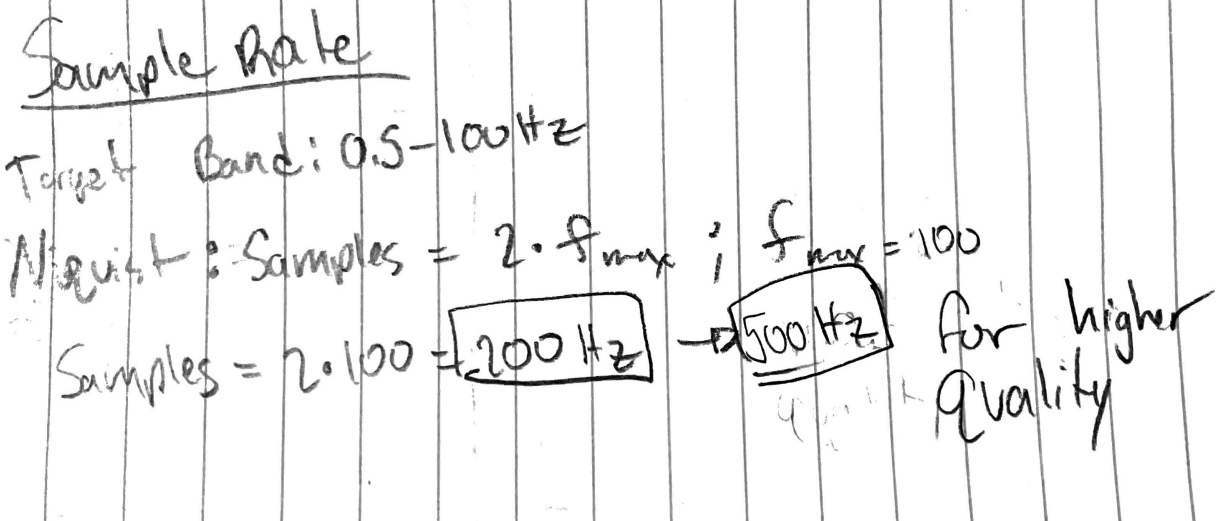
\includegraphics[width=3in, height=1in]{sample.png}
\end{figure}

\begin{figure}[h]
  \centering
  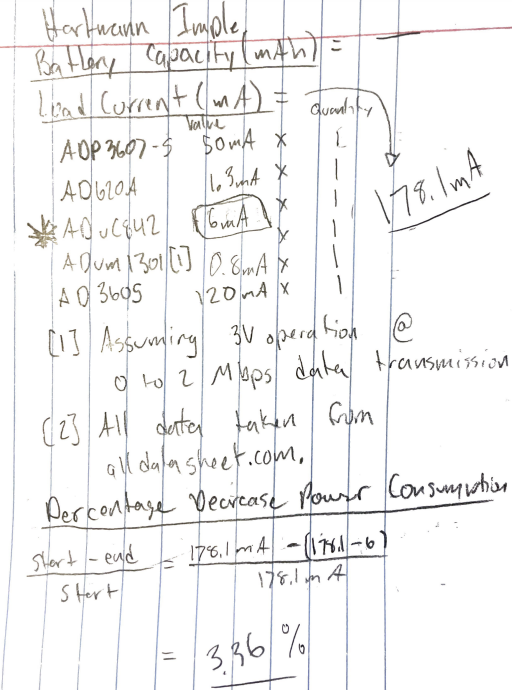
\includegraphics[width=3in, height=4in]{hartmann.png}
\end{figure}

\begin{figure}[h]
  \centering
  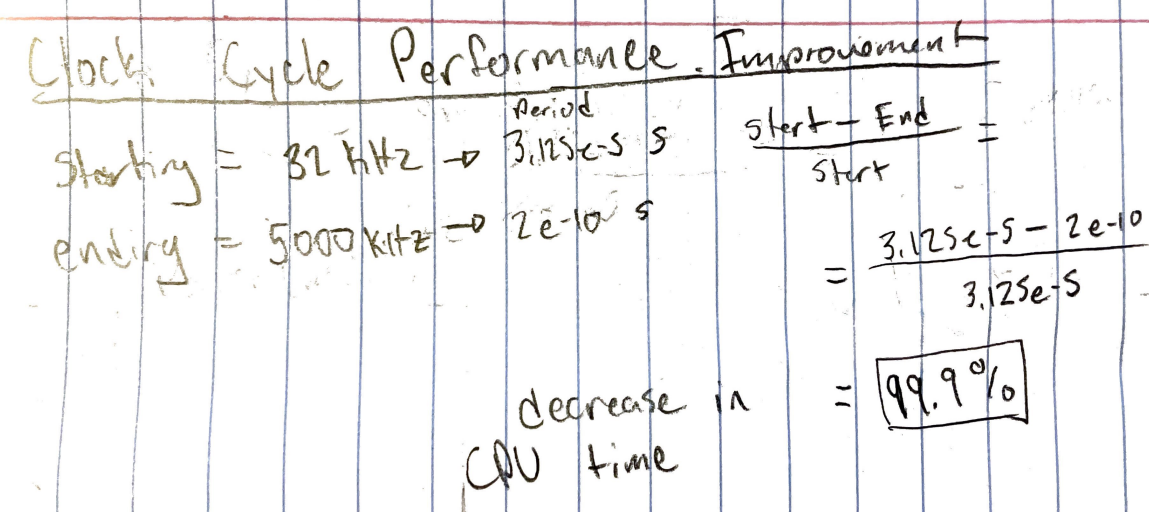
\includegraphics[width=3in, height=1.5in]{cpu.png}
\end{figure}

\end{document}